
\documentclass[aspectratio=169, 10pt]{beamer}
\usetheme{metropolis}
% Bundle fonts so XeLaTeX does not depend on operating-system font registration.
\usepackage{fontspec}
\setmainfont{Carlito}[Path=fonts/,Extension=.ttf,UprightFont=*-Regular,BoldFont=*-Bold,ItalicFont=*-Italic,BoldItalicFont=*-BoldItalic]
\setsansfont{Carlito}[Path=fonts/,Extension=.ttf,UprightFont=*-Regular,BoldFont=*-Bold,ItalicFont=*-Italic,BoldItalicFont=*-BoldItalic]
\setmonofont{DejaVuSansMono}[Path=fonts/,Extension=.ttf,UprightFont=*,BoldFont=*-Bold,ItalicFont=*-Oblique,BoldItalicFont=*-BoldOblique,Scale=0.82]
\newfontfamily\porson{GFSPorson.otf}[Path=fonts/]

\usepackage{booktabs}
\usepackage{tikz}
\usetikzlibrary{arrows.meta, positioning, shapes.misc, calc}
\usepackage{xcolor}
\usepackage{multicol}

\definecolor{ink}{HTML}{1F2A37}
\definecolor{aegean}{HTML}{5B2C83}
\definecolor{terracotta}{HTML}{B5533C}
\definecolor{olive}{HTML}{5B7F3B}
\definecolor{sand}{HTML}{F4EFE6}
\definecolor{mist}{HTML}{EEE8F4}
\definecolor{slate}{HTML}{6B7A8A}

\setbeamercolor{normal text}{fg=ink, bg=white}
\setbeamercolor{frametitle}{bg=aegean, fg=white}
\setbeamercolor{progress bar}{fg=terracotta, bg=mist}
\setbeamercolor{alerted text}{fg=terracotta}
\setbeamercolor{example text}{fg=olive}
\setbeamercolor{title separator}{fg=terracotta}
\setbeamercolor{block title}{bg=mist, fg=aegean}
\setbeamercolor{block body}{bg=sand, fg=ink}
\metroset{progressbar=frametitle, block=fill, numbering=fraction, sectionpage=progressbar}
\setbeamerfont{frametitle}{size=\large, series=\bfseries}
\setbeamertemplate{section in toc}[sections numbered]

\newcommand{\handoff}[1]{\vfill\begin{flushright}\footnotesize\textcolor{slate}{\textit{#1}}\end{flushright}}
\newcommand{\key}[1]{\textcolor{aegean}{\textbf{#1}}}
\newcommand{\hl}[1]{\textcolor{terracotta}{\textbf{#1}}}

\title{AI Applications for Language Analysis}
\subtitle{Instruments, analysts, and verifiers}
\author{Stergios Chatzikyriakidis}
\institute{ILSP}
\date{CLARIN:EL Summer School, 24 September 2026}

\begin{document}

\begin{frame}[plain,noframenumbering]
  \vspace{1em}
  {\LARGE\bfseries\inserttitle\par}
  \vspace{0.5em}
  {\large\insertsubtitle\par}
  \vspace{0.4em}{\color{terracotta}\rule{\textwidth}{1pt}}
  \vspace{0.7em}
  {\large\insertauthor\par}
  \insertinstitute\par
  \vspace{0.7em}\insertdate\par
  \small Language Technology and Artificial Intelligence for Digital Humanities
\end{frame}

\begin{frame}{Which AI?}
  \small Four families of methods, often used together. Name the configuration behind a result.
  \begin{columns}[T]
    \begin{column}{0.49\textwidth}
      \begin{block}{Symbolic: rules, logic, ontologies, proofs}
        \footnotesize Rhyme: Greek G2P and the Topintzi taxonomy.\\
        Zeugma: Prolog validates extracted events.\\
        RAG-to-Coq and semantics: proofs or refusals.\\
        HeptaTAX: discriminative legal formulae.\\
        TermGuard: ISO 1087-1 checks, alongside an LLM.
      \end{block}
      \begin{block}{Statistical and machine learning}
        \footnotesize Linguistic Distance and PhylProGramm: 16 languages, stability weights and phylogenies over ASJP, WALS, Grambank and UD. Perplexity: an LM's surprise as distance. Detectors: classifiers and probability scores.
      \end{block}
    \end{column}
    \begin{column}{0.49\textwidth}
      \begin{block}{Neural analysis: taggers and encoders}
        \footnotesize NATS and Voyant-NLP: spaCy entities, character networks and text statistics. RoBERTa: a trained detector.
      \end{block}
      \begin{block}{Generative language models}
        \footnotesize Claude, GPT-4o, Gemini, Llama and Krikri, plus prompts, retrieval, tools and verifiers.\\
        Rhyme, HeptaTAX, BookForge and chatbots: propose, draft and extract.\\
        A number belongs to the whole configuration.
      \end{block}
    \end{column}
  \end{columns}
  \footnotesize Much of the checking and measuring here uses symbolic rules or statistics.
\end{frame}

\begin{frame}{Three ways to put AI to work on language}
  \small
  \begin{columns}[T]
    \begin{column}{0.32\textwidth}
      \begin{block}{1. Instrument}
        The system \textbf{measures}.\\[2pt]
        Feature-based distance between Ancient and Modern Greek; perplexity as dialectal distance; detector scores as authorship evidence.
      \end{block}
    \end{column}
    \begin{column}{0.32\textwidth}
      \begin{block}{2. Analyst}
        The system \textbf{labels}.\\[2pt]
        Entities and character networks with spaCy; rhyme types, legal genres and historical events with LLMs.
      \end{block}
    \end{column}
    \begin{column}{0.32\textwidth}
      \begin{block}{3. Proposer and verifier}
        A model \textbf{proposes}, symbolic AI \textbf{verifies}.\\[2pt]
        Rules, gazetteers, logic programs, proof assistants.
      \end{block}
    \end{column}
  \end{columns}
  \vspace{1em}
  \centering
  \Large The question is the same in all three: \hl{how do we know it did it right?}\\[4pt]
  \normalsize The answer comes from the humanities. LLMs are one tool in the box, and rarely the one doing the checking.
\end{frame}

\begin{frame}{The frame: injective and federative neuro-symbolic systems}
  \small Chatzikyriakidis \& Lappin (2026), \emph{Neuro-symbolic NLP: taxonomy, assessment, and directions}. \emph{Frontiers in Artificial Intelligence}, \textbf{9}, article 1797587.
  \begin{columns}[T]
    \begin{column}{0.48\textwidth}
      \begin{block}{Injective}
        Symbolic structure is pushed \emph{inside} the network: as training signal, as architecture, as a loss.\\[2pt]
        Dominates the literature. Gains are usually marginal.
      \end{block}
    \end{column}
    \begin{column}{0.48\textwidth}
      \begin{block}{Federative}
        Neural and symbolic components stay \emph{separate} and exchange messages: the model proposes, a solver, a rule base or a proof assistant checks.\\[2pt]
        Fewer papers. Larger, more reliable gains. Not yet scaled to foundation-model size.
      \end{block}
    \end{column}
  \end{columns}
  \vspace{0.8em}
  \begin{itemize}
    \item Combined taxonomy: Kautz's composition codes plus Lappin's injective/federative distinction.
    \item Everything in Part III of this talk is federative. The symbolic side is where \key{your} knowledge goes.
  \end{itemize}
\end{frame}

\section{The model as instrument}

\begin{frame}{Perplexity as dialectal distance}
  \small
  \begin{columns}[T]
    \begin{column}{0.52\textwidth}
      \begin{itemize}
        \item \key{GRDD+}: 6.3M words, 10 Greek varieties (Chatzikyriakidis et al., 2026).
        \item Score each variety's text with a model. \textbf{Perplexity} is how surprised the model is by the text.
        \item The model's surprise \emph{ranks} varieties by their distance from the Greek it was trained on.
        \item Seven models, three sample sizes. The table shows eight varieties plus Standard Modern Greek.
      \end{itemize}
      \vspace{0.5em}
      \scriptsize Caveats: tokenisation drives the absolute numbers (Llama 2 splits Greek into 5--6 tokens per word, Krikri into 1.5--2.4); a distance is not a genealogy.
    \end{column}
    \begin{column}{0.44\textwidth}
      \centering
      \footnotesize
      \begin{tabular}{lr}
        \toprule
        \textbf{Variety} & \textbf{PPL, Krikri-8B} \\
        \midrule
        Standard Modern Greek & 8.8 \\
        Heptanesian & 12.4 \\
        Cypriot & 24.7 \\
        Maniot & 24.7 \\
        Pontic & 37.2 \\
        Northern & 41.6 \\
        Cretan & 62.1 \\
        Tsakonian & 96.5 \\
        Griko & 121.6 \\
        \bottomrule
      \end{tabular}\\[3pt]
      \tiny 25,000-word samples.
    \end{column}
  \end{columns}
  \handoff{What to do about the distance: Markantonatou, Bompolas, Stamou \& Dimakis, today 11:30}
\end{frame}

\begin{frame}{PhylProGramm: measuring 2,500 years of change}
  \begin{columns}[T]
    \begin{column}{0.55\textwidth}
      \begin{itemize}
        \item Sixteen Indo-European languages in ancient-to-modern pairs: Ancient $\rightarrow$ Modern Greek, Latin $\rightarrow$ Romance, Old Church Slavonic $\rightarrow$ Slavic, Gothic $\rightarrow$ German, Sanskrit $\rightarrow$ Hindi.
        \item Seven dimensions of distance, each from a curated resource.
        \item Stability-based weighting (F-ratio): which features resist change across the transitions?
        \item Distance-based and character-based phylogenies, with uncertainty quantification.
      \end{itemize}
      \vspace{0.4em}
      \tiny Funded by the European Union (ERC AdG PhylProGramm, grant 101096554). [VERIFY wording]
    \end{column}
    \begin{column}{0.42\textwidth}
      \centering
      \small
      \begin{tabular}{ll}
        \toprule
        \textbf{Dimension} & \textbf{Resource} \\
        \midrule
        lexical & Swadesh lists \\
        typological & WALS, Grambank \\
        featural & URIEL \\
        syntactic & UD treebanks \\
        phonological & ASJP \\
        cognates & CLDF cognate sets \\
        \bottomrule
      \end{tabular}
    \end{column}
  \end{columns}
\end{frame}

\begin{frame}{What resists change}
  \begin{columns}[T]
    \begin{column}{0.55\textwidth}
      \begin{itemize}
        \item \key{Cognate distance} carries 48\% of the stability-based weight. The comparative method, vindicated by the numbers.
        \item Only \key{26 of 72} WALS features change in fewer than 20\% of the historical transitions.
        \item \key{Six} features never changed in the sample, among them adposition order and possessive marking.
        \item Family-specific: case marking is stable in Slavic and unstable in Romance.
      \end{itemize}
    \end{column}
    \begin{column}{0.42\textwidth}
      \begin{block}{Lesson}
        ``AI for language analysis'' is not only large language models. Curated databases plus statistics answer questions no LLM can, and they say what they measure.
      \end{block}
    \end{column}
  \end{columns}
\end{frame}

\begin{frame}{Detection as authorship attribution}
  \begin{itemize}
    \item The oldest question in philology: \emph{who wrote this?} The 2026 version: \emph{was it a model?}
    \item \key{Corpus}: 1,550 baseline texts from eight model families (GPT-4o, GPT-5.5, Llama 3.3 70B, Mistral Large 3, DeepSeek V4 Pro, Kimi K2.6, Phi-4 reasoning, Grok 4.1) plus a human reference corpus.
    \item \key{Perturbation}: round-trip machine translation, en $\rightarrow$ X $\rightarrow$ en, pivots fr, el, zh, ja, ar, and double hops (en $\rightarrow$ X $\rightarrow$ ja $\rightarrow$ en). 13,950 round trips in the supplied results.
    \item \key{Detectors}: Binoculars (perplexity ratio) and Fast-DetectGPT (probability curvature), both zero-shot and a fine-tuned RoBERTa classifier, an encoder, not a generative model.
    \item \key{Calibration}: true-positive rate at a fixed false-positive rate on the human corpus. A detector that flags humans is not a detector.
  \end{itemize}
\end{frame}

\begin{frame}{What a detector measures}
  \footnotesize
  \setlength{\parskip}{0pt}
  \begin{columns}[T]
    \begin{column}{0.5\textwidth}
      \centering
      \scriptsize
      Texts by Llama 3.3 70B, true-positive rate\\[3pt]
      \begin{tabular}{lrr}
        \toprule
        \textbf{Condition} & \textbf{Binoculars} & \textbf{RoBERTa} \\
        \midrule
        original & 93\% & 57\% \\
        en$\to$fr$\to$en & 85\% & 57\% \\
        en$\to$el$\to$en & 82\% & 59\% \\
        en$\to$zh$\to$en & 54\% & 42\% \\
        en$\to$ja$\to$en & 50\% & 45\% \\
        en$\to$ar$\to$ja$\to$en & \hl{26\%} & 43\% \\
        \bottomrule
      \end{tabular}\\[3pt]
    \end{column}
    \begin{column}{0.48\textwidth}
      \footnotesize
      \begin{itemize}
        \item Evasion \textbf{scales with typological distance} of the pivot and with hop count.
        \item Probability-based detectors measure ``how model-like is this surface''. Translation rewrites the surface.
        \item The trained classifier does not collapse: it picks up something translation preserves. Joint evasion needs paired predictions [VERIFY].
        \item English-only detector performance on Greek requires a separate evaluation [VERIFY].
      \end{itemize}
      \begin{block}{For the humanities}
        A detector score is a measurement with a theory behind it. Know the theory before trusting the number.
      \end{block}
    \end{column}
  \end{columns}
\end{frame}

\section{The model as analyst}

\begin{frame}{Rhyme in Modern Greek: the task}
  \footnotesize
  \begin{columns}[T]
    \begin{column}{0.5\textwidth}
      \textbf{By stress position} (Topintzi et al., 2019)
      \begin{itemize}
        \item M, oxytone: καρδιά / φωτιά
        \item F2, paroxytone: ελπίδα / πατρίδα
        \item F3, proparoxytone: στόματα / σώματα
      \end{itemize}
      \textbf{Independent features}
      \begin{itemize}
        \item Rich: onset of the stressed syllable matches (καλά / μαλά)
        \item IDV: the pre-stress vowel matches (ξανθή / γραφή)
        \item Mosaic: the rhyme domain spans a word boundary (όνομά της / ο μπάτης)
        \item Imperfect: systematic vowel or consonant variation (χάνετε / γίνετε); Copy: same lemma
      \end{itemize}
    \end{column}
    \begin{column}{0.46\textwidth}
      \begin{itemize}
        \item The domain is the \textbf{phonological word}: a host plus its weak pronoun. The three-syllable rule applies.
        \item A token-based model sees letters in chunks; rhyme lives in syllables, stress and sound.
        \item \key{Corpus}: 40,000+ rhymes from the Anemoskala and Interwar Poetry corpora, cleaned and released.
      \end{itemize}
      \vspace{0.3em}
      \scriptsize Chatzikyriakidis \& Natsina, \emph{LLMs Got Rhyme? Hybrid Phonological Filtering for Greek Poetry Rhyme Detection and Generation}, LaTeCH-CLfL 2026 (EACL). Code: \texttt{github.com/StergiosCha/Greek\_Rhyme}
    \end{column}
  \end{columns}
\end{frame}

\begin{frame}{What models hear}
  \small
  \begin{columns}[T]
    \begin{column}{0.5\textwidth}
      \centering
      \footnotesize
      Identification accuracy, best configuration per model\\[3pt]
      \begin{tabular}{lrl}
        \toprule
        \textbf{Model} & \textbf{Acc.} & \textbf{Needs} \\
        \midrule
        Claude 4.5 & 53.8\% & CoT + RAG \\
        GPT-4o & 50.0\% & CoT (7.7\% without) \\
        Claude 3.7 & 42.3\% & RAG or CoT \\
        Gemini 2.0 & 42.3\% & RAG \\
        Mistral Large & 26.9\% & CoT \\
        Llama 3.1 8B & 15.4\% & RAG \\
        \bottomrule
      \end{tabular}\\[6pt]
      By stress, Claude 4.5: M 65.6\%, F2 47.5\%, \hl{F3 21.9\%}
    \end{column}
    \begin{column}{0.48\textwidth}
      \begin{itemize}
        \item \textbf{F3} (proparoxytone) is the hardest for every model.
        \item \textbf{Mosaic} rhymes: \hl{0\%} across all models and prompts. These tested configurations missed rhyme domains crossing word boundaries.
        \item Homophones flagged as copies: κρίνοι / κρίνει, ``lilies'' and ``judges'', judged the same word.
        \item GPT-4o: 7.7\% to 50\% with chain-of-thought. It knows more than it lets on, but must be walked through it.
        \item \textbf{Everyone in this room can see these errors without a leaderboard.}
      \end{itemize}
    \end{column}
  \end{columns}
\end{frame}

\begin{frame}{Generation: propose, verify, refine}
  \begin{columns}[T]
    \begin{column}{0.5\textwidth}
      \centering
      \footnotesize
      Valid poems, rhyme constraints fully satisfied\\[3pt]
      \begin{tabular}{lrr}
        \toprule
        \textbf{Model} & \textbf{Alone} & \textbf{With verifier loop} \\
        \midrule
        Claude 3.7 & 3.8\% & \hl{73.1\%} \\
        GPT-4o & 0.0\% & 42.3\% \\
        Claude 4.5 & 0.0\% & 34.6\% \\
        \bottomrule
      \end{tabular}
      \vspace{1.2em}
      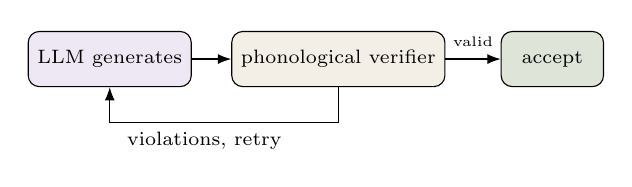
\begin{tikzpicture}[node distance=5mm, every node/.style={font=\scriptsize}]
        \node[draw, rounded corners, fill=mist, minimum width=1.9cm, minimum height=7mm] (gen) {LLM generates};
        \node[draw, rounded corners, fill=sand, minimum width=2.1cm, minimum height=7mm, right=5mm of gen] (ver) {phonological verifier};
        \node[draw, rounded corners, fill=olive!20, minimum width=1.3cm, minimum height=7mm, right=7mm of ver] (ok) {accept};
        \draw[-Latex] (gen) -- (ver);
        \draw[-Latex] (ver) -- node[above=1pt, font=\tiny]{valid} (ok);
        \draw[-Latex] (ver.south) |- ++(-0.5,-0.45) -| node[below, pos=0.25]{violations, retry} (gen.south);
      \end{tikzpicture}
    \end{column}
    \begin{column}{0.48\textwidth}
      \begin{itemize}
        \item Ask for a poem with a rhyme scheme and features: almost nothing comes back fully valid.
        \item Add a deterministic verifier (Greek grapheme-to-phoneme rules plus the taxonomy) and loop on its report.
        \item The verifier is a 2019 linguistics paper turned into code. No training.
        \item Still unsolved: combinations such as IDV + mosaic stay at 0\% even with the loop.
      \end{itemize}
    \end{column}
  \end{columns}
\end{frame}

\begin{frame}{HeptaTAX: notarial acts of sixteenth-century Corfu}
  \small
  \begin{columns}[T]
    \begin{column}{0.5\textwidth}
      \begin{itemize}
        \item \key{1,088 acts} by five Corfiot notaries, 1500--1567; editions digitised at the Laboratory of Southeastern Mediterranean Linguistics (Aegean).
        \item Non-standard orthography, Greek/Latin/Italian code-switching, formulaic but variable legal language.
        \item \key{Three tiers}: 17 core genres (Venditio, Testamentum, Emphyteusis, \ldots), extensions, hybrid tags. 40-act gold benchmark.
        \item Twelve LLMs $\times$ four settings: zero-shot, few-shot, full-context, \textbf{neuro-symbolic}.
        \item[] \textcolor{slate}{\textit{After the image becomes text (Gatos, 14:30), this is the next step.}}
      \end{itemize}
    \end{column}
    \begin{column}{0.48\textwidth}
      \begin{block}{The symbolic engine}
        Deterministic rules detect the discriminative legal formulae; their output goes into the prompt. The model may override.
      \end{block}
      \begin{itemize}
        \item Gap between strongest and weakest model: \hl{47.5 $\rightarrow$ 12.5 points}.
        \item Llama 3.1 8B gains 47.5 points and matches frontier models running without symbolic support.
        \item Ceiling on the core tier: 72.5\%. Extensions about 63\%, hybrids about 35\%.
        \item Errors cluster in procedurally dense acts: lexical cues do not identify \emph{legal effect}.
      \end{itemize}
    \end{column}
  \end{columns}
\end{frame}

\begin{frame}{More analysts, same lesson}
  \small
  \setlength{\parskip}{2pt}
  \begin{itemize}
    \item \key{NATS}: entities, character networks and text statistics for Greek literature with spaCy. No LLM, no invented entities, its own error profile.
    \item \key{Greek parliamentary speech}: stance and rhetoric at scale, labels audited (doctoral work under supervision).
    \item \key{Curriculum compliance}: scoring textbooks against the curriculum by thematic field, from the ministry's PDFs.
    \item \key{OYXOY NLI} and \emph{Reverse-Engineering NLI} (COLM 2025): models pass benchmarks by routes never intended.
    \item \key{Gender bias in Greek pronoun resolution} (Llama, Krikri): the analyst has priors. \textit{Friday, Gkirtzou.}
    \item \key{Interpretable mixture of experts} for dialect text: which expert fires on which feature. \textit{Friday, Paraskevopoulos.}
  \end{itemize}
  \begin{block}{Common thread}
    A label from a model is a hypothesis. It becomes a finding when a philologist, a rule, or a benchmark with teeth has checked it.
  \end{block}
\end{frame}

\section{The model as proposer, the humanities as verifier}

\begin{frame}{The pattern}
  \centering
  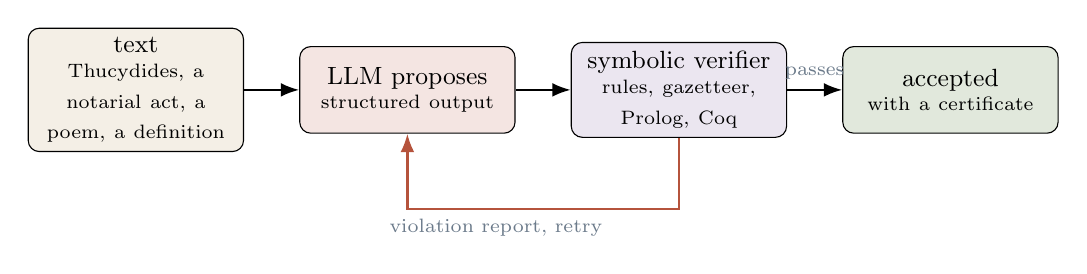
\begin{tikzpicture}[
      node distance=9mm and 7mm,
      box/.style={draw, rounded corners, minimum height=11mm, text width=2.5cm, align=center, font=\small},
      lab/.style={font=\scriptsize, text=slate}
    ]
    \node[box, fill=sand] (txt) {text\\[-2pt]{\scriptsize Thucydides, a notarial act, a poem, a definition}};
    \node[box, fill=terracotta!15, right=of txt] (llm) {LLM proposes\\[-2pt]{\scriptsize structured output}};
    \node[box, fill=aegean!12, right=of llm] (ver) {symbolic verifier\\[-2pt]{\scriptsize rules, gazetteer, Prolog, Coq}};
    \node[box, fill=olive!18, right=of ver] (out) {accepted\\[-2pt]{\scriptsize with a certificate}};
    \draw[-Latex, thick] (txt) -- (llm);
    \draw[-Latex, thick] (llm) -- (ver);
    \draw[-Latex, thick] (ver) -- node[lab, above]{passes} (out);
    \draw[-Latex, thick, terracotta] (ver.south) |- ++(-1.2,-0.9) -| node[lab, below, pos=0.25]{violation report, retry} (llm.south);
  \end{tikzpicture}
  \vspace{1em}
  \begin{columns}[T]
    \begin{column}{0.48\textwidth}
      \begin{itemize}
        \item Federative: the two sides never share weights.
        \item The verifier cannot be charmed by fluent prose.
      \end{itemize}
    \end{column}
    \begin{column}{0.48\textwidth}
      \begin{itemize}
        \item The verifier encodes a taxonomy, a gazetteer, a chronology, a definition theory.
        \item That is \key{your} knowledge, written so a machine can refuse.
      \end{itemize}
    \end{column}
  \end{columns}
\end{frame}

\begin{frame}{Zeugma: reasoning over Thucydides}
  \begin{columns}[T]
    \begin{column}{0.55\textwidth}
      \begin{itemize}
        \item Task: extract events from the \emph{History} as RDF (actor, action, place, year); enrich with Wikidata, DBpedia and ConceptNet; resolve places to coordinates.
        \item Model RDF is dirty: duplicate identifiers, malformed literals, ``Here are the events\ldots'' preambles. Apache Jena parses \hl{0 of 32} outputs.
        \item \key{Zeugma}: fault-tolerant parser (53\% strict, 100\% in recovery mode), RDF $\rightarrow$ Prolog, user-defined rules. 12$\times$ faster than Jena.
        \item Claude Sonnet 4, GPT-4o, Llama 70B, Llama 8B, eight extraction configurations each.
      \end{itemize}
    \end{column}
    \begin{column}{0.43\textwidth}
      \begin{block}{Why this text}
        Precisely dated, densely located, argued: a stress test for keeping events, places and years consistent.
      \end{block}
      {\porson\small κτῆμά τε ἐς αἰεὶ μᾶλλον ἢ ἀγώνισμα ἐς τὸ παραχρῆμα ἀκούειν ξύγκειται.} {\scriptsize (1.22)}\\[4pt]
      \footnotesize Workshop interface in MEDEA-NEUMOUSA. Paper venue: CLASP Concluding Conference.
    \end{column}
  \end{columns}
\end{frame}

\begin{frame}{Rules catch what syntax cannot}
  \begin{columns}[T]
    \begin{column}{0.48\textwidth}
      \begin{block}{A temporal rule in Prolog}
        \texttt{suspicious\_date(E, Y) :-}\\
        \texttt{\ \ hasYear(E, S), atom\_number(S, Y),}\\
        \texttt{\ \ Y > -100, Y < 0.}\\[4pt]
        \footnotesize ``Battle of Sybota in year $-8$'': a well-formed triple, an impossible date.
      \end{block}
      \begin{block}{Negation as failure}
        Missing locations can be tested with Prolog negation or SPARQL \texttt{FILTER NOT EXISTS}. Prolog also supports conditional recursive rules.
      \end{block}
    \end{column}
    \begin{column}{0.48\textwidth}
      \begin{itemize}
        \item 333 catalogued errors (13 temporal, 290 geographic, 30 agency). Full detection claim [VERIFY]; the paper reports no false positives on clean data.
        \item Simulated self-correction: a violation report motivates changing ``2024'' to $-433$ for Sybota. The supplied demonstration scripts the correction.
      \end{itemize}
      \begin{block}{The point}
        The rules are the historian's knowledge: chronology, geography, who can act on whom. The model never sees them as weights.
      \end{block}
    \end{column}
  \end{columns}
\end{frame}

\begin{frame}{RAG-to-Coq: from events to proofs}
  \begin{columns}[T]
    \begin{column}{0.55\textwidth}
      \begin{itemize}
        \item Same source, stronger verifier: extracted events become \textbf{Coq propositions}, and the proof assistant checks their consistency with what is already established.
        \item Five configurations to see what each component buys: \textbf{zero-shot}, \textbf{base}, \textbf{KG-only}, \textbf{RAG-only}, \textbf{full}.
        \item Token-aware chunking, multi-knowledge-graph integration, caching; an interactive proving interface with the live goal state.
      \end{itemize}
    \end{column}
    \begin{column}{0.43\textwidth}
      \begin{block}{Why a proof assistant}
        A proof either closes or it does not. There is no partial credit, no fluent wrong answer, and the certificate can be inspected by someone who does not trust the model.
      \end{block}
      \begin{block}{Why it matters for a historian}
        The pipeline is forced to say which claims it relies on. That is a bibliography, mechanised.
      \end{block}
    \end{column}
  \end{columns}
\end{frame}

\begin{frame}{TermGuard: Aristotle as a validator}
  \begin{columns}[T]
    \begin{column}{0.5\textwidth}
      \begin{itemize}
        \item ISO 1087-1: a definition names the \textbf{genus} (the superordinate concept) and the \textbf{differentiae}. Definition by genus and differentia: \emph{Topics}, \emph{Posterior Analytics}.
        \item \key{TermGuard} checks a candidate definition: is the genus a recognised concept (grounded in open lexical and ontological resources)? Is it circular? Do the differentiae distinguish?
        \item Then terminology-aware translation and export as TBX (ISO 30042), for Greek and the other EU languages.
      \end{itemize}
    \end{column}
    \begin{column}{0.48\textwidth}
      \begin{block}{The proposer}
        A model drafts terms, equivalents and definitions from domain text.
      \end{block}
      \begin{block}{The verifier}
        A definitional theory 2,300 years older than the technology, plus a reference termbase built only from authoritative, licensed, machine-readable collections.
      \end{block}
    \end{column}
  \end{columns}
\end{frame}

\begin{frame}{BookForge: the pattern at production scale}
  \begin{itemize}
    \item Greek children's picture books: \textbf{story bible} $\rightarrow$ \textbf{drafting board with critics} $\rightarrow$ \textbf{symbolic validation} $\rightarrow$ reference-conditioned illustration $\rightarrow$ PDF in publishing-house presets (Οσελότος, Υδροπλάνο, \ldots).
    \item «Το Σχολείο μέσα στο Παραμύθι»: exercises per primary-school grade, aligned with the curriculum, grounded in the story. Every arithmetic answer is \textbf{computed by code}, not by the model.
    \item An author's own story can be imported verbatim: the pipeline then does illustration and layout only.
    \item Built on Azure Foundry models; the critics and validators are the same propose-and-verify loop as the rhyme system, one level up.
  \end{itemize}
  \begin{block}{Same pattern, different verifier}
    Rhymes: a phonological rule set. Thucydides: Prolog and Coq. Terms: ISO 1087-1. Children's books: continuity checks, vocabulary level, a calculator.
  \end{block}
\end{frame}

\begin{frame}{Formalising semantics in Coq: the rigor gap}
  \begin{columns}[T]
    \begin{column}{0.52\textwidth}
      \begin{itemize}
        \item A Coq library mechanising influential papers in formal semantics: 31 files, more than 235 theorems.
        \item Montague, Kratzer, Rooth, Dowty, Link, Champollion, Barwise \& Cooper, MTT adjectives and mass/count, Greek polydefinites, presupposition projection, DPL.
        \item \textbf{File Change Semantics} resists mechanisation: non-determinism, global state, implicit choices.
      \end{itemize}
    \end{column}
    \begin{column}{0.46\textwidth}
      \begin{block}{What formalisation shows}
        What a theory actually commits to. Kratzer's modal semantics turns out to be an interface to existing modal logic rather than new machinery. Some ``formal'' semantics is less formal than it looks.
      \end{block}
      \begin{block}{A method for the humanities}
        Write the theory down so a machine can refuse it. The refusals are the findings.
      \end{block}
    \end{column}
  \end{columns}
\end{frame}

\section{Reaching people}

\begin{frame}{When grounding is a safety requirement}
  \begin{columns}[T]
    \begin{column}{0.5\textwidth}
      \textbf{SimasiaAI, Greek-language applications}
      \begin{itemize}
        \item Assistant for ΚΑΠΑ3 (cancer patient guidance centre): oncology patients' social and welfare rights. Delivered free.
        \item BPAN Companion, for a rare-disease patient association (pro bono).
        \item Assistant for the multiple-sclerosis patient federation (ΠΟΑμΣΚΠ).
        \item SimasiaEdu for tutoring centres; DialogosAI.
      \end{itemize}
    \end{column}
    \begin{column}{0.48\textwidth}
      \begin{block}{The constraint}
        A wrong answer about a welfare deadline hurts a real person. So: retrieval over verified documents only, refusal when the sources do not support an answer, and people in the loop.
      \end{block}
      \begin{itemize}
        \item The same architecture as Part III, with a human as the last verifier.
        \item EU AI Act compliance is a design input, not an afterthought.
      \end{itemize}
    \end{column}
  \end{columns}
\end{frame}

\begin{frame}{Takeaways, and where the day goes next}
  \begin{columns}[T]
    \begin{column}{0.55\textwidth}
      \begin{enumerate}
        \item \key{Instrument}: know what the number measures. Perplexity measures surprise; a detector measures surface likeness to a model.
        \item \key{Analyst}: the label is a hypothesis. Verify it with something that cannot be charmed.
        \item \key{Proposer}: let the model propose; let a rule, a gazetteer, a proof assistant, or a philologist decide.
        \item ``AI'' is four families of methods. Name the one you used. Most checking and measuring here is symbolic or statistical.
      \end{enumerate}
      \vspace{0.5em}
      \Large\centering \hl{Your expertise is the verifier.}
    \end{column}
    \begin{column}{0.43\textwidth}
      \begin{block}{Today}
        11:30 Low-resource varieties: Markantonatou, Bompolas, Stamou, Dimakis\\
        12:15 Ancient Greek: Platanou\\
        14:30 Historical document images: Gatos
      \end{block}
      \begin{block}{Friday}
        Social biases: Gkirtzou\\
        Explainability: Paraskevopoulos
      \end{block}
    \end{column}
  \end{columns}
\end{frame}

\begin{frame}{Everything here is live}
  \begin{columns}[T]
    \begin{column}{0.5\textwidth}
      \textbf{Greek NLP Swiss Knife} (Azure Container Apps)
      \begin{itemize}
        \item MEDEA-NEUMOUSA, with Zeugma and the knowledge-graph extractor
        \item Greek Rhyme System
        \item TermGuard
        \item Dialect Generator
        \item Linguistic Distance
        \item NATS, PlotAnalyzer, Voyant-NLP
      \end{itemize}
    \end{column}
    \begin{column}{0.46\textwidth}
      \textbf{Svarna} lab site
      \begin{itemize}
        \item Greek Corpus Workbench
        \item Datasets: GRDD+, OYXOY, the rhyme corpus
        \item One page that links every demo
      \end{itemize}
    \end{column}
  \end{columns}
  \vspace{0.8em}
  \centering
  Entry point: \href{https://stergioscha.github.io/svarna/demos.html}{\nolinkurl{stergioscha.github.io/svarna/demos.html}}\\[4pt]
  You can keep using all of this after Thursday. The workshop apps provide access; an external chat comparison can use your existing account.
\end{frame}

\begin{frame}{Hands-on, 10:15}
  \small
  \begin{columns}[T]
    \begin{column}{0.48\textwidth}
      \begin{block}{A. The analyst who cannot hear (15 min)}
        Paste a stanza of Solomos into a chat model and ask for the rhyme types. Then run it through the Greek Rhyme System. Find the stress and mosaic errors yourselves.
      \end{block}
    \end{column}
    \begin{column}{0.48\textwidth}
      \begin{block}{B. Propose, then verify (25 min)}
        Pick a passage of Thucydides on the Zeugma page of MEDEA-NEUMOUSA. A model extracts events; Prolog rules check chronology, geography and agency. Read the violation report. Feed it back and check whether the next graph improves.
      \end{block}
    \end{column}
  \end{columns}
  \vspace{0.8em}
  \centering
  Start here: \href{https://stergioscha.github.io/svarna/demos.html}{\nolinkurl{stergioscha.github.io/svarna/demos.html}}\\[4pt]
  Workshop access is provided in your browser.\\[3pt]
  \footnotesize\href{https://greek-app-heaven-rhyme.livelyhill-85880e66.westeurope.azurecontainerapps.io}{A: Greek Rhyme System}
  \quad\href{https://greek-app-heaven-medea.livelyhill-85880e66.westeurope.azurecontainerapps.io/zeugma}{B: MEDEA Zeugma}
  \vspace{0.6em}
  \begin{flushleft}\footnotesize If time remains: the Dialect Generator (write a Cretan sentence, judge it) and Linguistic Distance (Ancient to Modern Greek across dimensions), as a bridge to 11:30.\end{flushleft}
\end{frame}

\begin{frame}[standout]
  Thank you\\[1em]
  {\normalsize\normalfont
  stergios.chatzikyriakidis@uoc.gr\\[2pt]
  {\scriptsize Preferred contact [VERIFY]}\\[4pt]
  \texttt{stergioscha.github.io/svarna}}\par\vspace{1em}
  {\small\normalfont
  \textbf{Funding acknowledgment}\par\vspace{5pt}
  \begin{minipage}{.92\textwidth}
    \centering Funding from Microsoft's LINGUA project supported CoDAG (Computational Dialectal Atlas of Greek), making Svarna, GPT-4.1 fine-tuning and the Greek NLP Swiss Knife possible.
  \end{minipage}}
\end{frame}

\end{document}
